\section{Specification and Design}
\label{sec:design}

\begin{guidance}[Specification and design (15 marks)]
Required (brief, A.3--A.5): an \textbf{embedded server FSM} covering IDLE,
IN\_PROGRESS, GAME\_OVER \textbf{and the move-validation branch}; a
\textbf{flowchart of the GUI application}; and a \textbf{circuit diagram} of the
STM-to-PC UART connection, with the on-board button and LED behaviour labelled.
Diagrams may be at function level. Explain \textbf{why} responsibilities sit on
the server or the client. Draw diagrams in a tool that exports vector PDF
(draw.io, TikZ, Mermaid) and check that every label is readable when printed.
\end{guidance}

\subsection{The server decides; the client only draws}
Table~\ref{tab:owner} assigns each decision to one side. The server holds the
only copy of the game state (the board, the side to move and the game status)
and the client never computes any of it. The firmware has two layers. Hardware
code covers the USART interrupt, polled transmit, the LED and the button.
Rule code covers \texttt{check\_win}, \texttt{check\_draw},
\texttt{handle\_move} and the command dispatcher, which depend only on the
game variables and on \texttt{send\_str}. I kept the rules apart from the
interrupt and LED code so that they never depend on timing.

\begin{table}[t]
\centering
\caption{Who owns each decision.}
\label{tab:owner}
\footnotesize
\begin{tabular}{@{}L{3.5cm}L{1.3cm}L{3.0cm}@{}}
\toprule
Decision & Owner & Why \\
\midrule
Board, turn, game status & server & one source of truth \\
Is a move legal? & server & a client cannot be trusted \\
Win and draw detection & server & result must match the LED \\
Session (\texttt{CONNECT}) & server & rejects commands before it \\
What is drawn & client & only from \texttt{OK:BOARD}, \texttt{BOARD} \\
AI move choice & server & same write path as a human \\
Move history, undo & server & client keeps no move list \\
LED and button & server & board-side indicators \\
\bottomrule
\end{tabular}
\end{table}

\subsection{Three states and a validation chain that writes last}
Figure~\ref{fig:fsm} shows the server FSM. In IDLE the server accepts
\texttt{NEW} (or \texttt{NEW:AI}) once a session is open. In IN\_PROGRESS it accepts
\texttt{MOVE}, \texttt{STATE}, \texttt{HISTORY}, \texttt{UNDO} and \texttt{RESIGN}; a legal
move stays in IN\_PROGRESS unless it wins or fills the board. In GAME\_OVER it accepts
\texttt{NEW}, \texttt{STATE} and \texttt{HISTORY}, and a \texttt{MOVE} or \texttt{UNDO} gets
\texttt{NACK:NOGAME}. \texttt{DISCONNECT} returns any
state to IDLE. The lower part of the figure expands the validation branch. The
five checks come before the first write to the board, so every
\texttt{NACK} exit leaves the state unchanged. The figure omits the
\texttt{NOCONN}, \texttt{TOOLONG}, \texttt{TIMEOUT} and \texttt{CHECKSUM} replies, which belong
to the framer and the session check and never reach the state machine.

\begin{figure*}[t]
\centering
\begin{tikzpicture}[font=\scriptsize,>=Stealth,
  st/.style={draw,rounded corners=3pt,minimum width=2.6cm,minimum height=0.9cm,fill=blue!7,thick},
  bx/.style={draw,minimum width=1.95cm,minimum height=1.0cm,text width=1.85cm,align=center,fill=gray!8},
  nk/.style={draw,rounded corners=2pt,fill=red!9,font=\tiny\ttfamily,minimum width=1.7cm,minimum height=0.55cm,align=center},
  ok/.style={draw,rounded corners=2pt,fill=green!10,font=\tiny\ttfamily,minimum width=1.7cm,minimum height=0.55cm,align=center},
  ar/.style={->,line width=0.5pt}]
  % ---- states
  \node[st] (idle) at (1.6,0) {IDLE};
  \node[st] (prog) at (9.1,0) {IN\_PROGRESS};
  \node[st] (over) at (16.6,0) {GAME\_OVER};
  \draw[ar] (idle.east) -- node[above,align=center]{\texttt{NEW}, \texttt{NEW:AI} (session open)\\ / \texttt{OK:BOARD}} (prog.west);
  \draw[ar] (prog.east) -- node[above,align=center]{\texttt{MOVE} wins / \texttt{WIN:m}\\\texttt{MOVE} fills / \texttt{DRAW}\\\texttt{RESIGN} / \texttt{OK:GAMEOVER}} (over.west);
  \draw[ar] (prog.70) to[out=70,in=110,looseness=8]
     node[above,align=center]{legal \texttt{MOVE}, \texttt{UNDO} / \texttt{OK:BOARD}; \texttt{STATE} / \texttt{BOARD}; \texttt{HISTORY} / \texttt{HIST}\\any rejected request / \texttt{NACK} (state unchanged)} (prog.110);
  \draw[ar] (over.south west) .. controls +(-2.2,-1.5) and +(2.2,-1.5) .. node[below,pos=0.5]{\texttt{NEW} / \texttt{OK:BOARD}} (prog.south east);
  \draw[ar] (prog.south west) .. controls +(-2.2,-1.5) and +(2.2,-1.5) .. node[below,pos=0.5,align=center]{\texttt{DISCONNECT} (any state) / \texttt{OK}\\closes the session} (idle.south east);
  \node[draw,dashed,align=center,fill=yellow!10] (btn) at (14.6,2.3) {Button SW0 (session open):\\\texttt{game\_new()} + unsolicited \texttt{OK:BOARD}};
  \draw[ar,dashed] (btn.west) -- (prog.30);
  % ---- validation chain
  \node[font=\footnotesize\bfseries,anchor=west] at (0.2,-3.0) {\texttt{MOVE} validation branch (runs inside IN\_PROGRESS)};
  \foreach \i/\t in {0/{state is\\IN\_PROGRESS?},1/{parse\\\texttt{MOVE:<i>} or\\\texttt{MOVE:<i>:<m>}},2/{index\\in 0 to 8?},3/{mark equals\\turn (if given)?},4/{cell\\empty?},5/{place mark;\\win? board full?},6/{swap turn;\\AI mode: AI\\moves too}} {
    \node[bx] (b\i) at ({1.25+2.5*\i},-4.4) {\t};
  }
  \foreach \i/\j in {0/1,1/2,2/3,3/4,4/5,5/6} {\draw[ar] (b\i) -- (b\j);}
  \foreach \i/\t in {0/NACK:NOGAME,1/NACK:BADCMD,2/NACK:RANGE,3/NACK:NOTURN,4/NACK:OCCUPIED} {
    \draw[ar,red!60!black] (b\i.south) -- ++(0,-0.55) node[nk,anchor=north] {\t};
  }
  \draw[ar] (b5.south) -- ++(0,-0.55) node[ok,anchor=north,font=\tiny\ttfamily,text width=1.7cm] {WIN:m or DRAW};
  \draw[ar] (b6.south) -- ++(0,-0.55) node[ok,anchor=north] {OK:BOARD};
  \draw[thick,gray] (0.3,-3.55) -- node[above]{no state written on any exit} (11.4,-3.55);
  \draw[thick,gray] (11.6,-3.55) -- node[above]{state written} (16.9,-3.55);
\end{tikzpicture}

\caption{Server FSM with the move-validation branch. Red exits are NACKs
that leave the state unchanged; green exits are successes. The symbol
\texttt{m} stands for the mark of the side to move.}
\label{fig:fsm}
\end{figure*}

\subsection{The GUI never blocks and never guesses}
Figure~\ref{fig:gui} shows the client flow. A reader thread blocks on the port and
puts each line into a queue; the Tk main loop empties the queue every 50~ms, so the
window stays responsive. After the port opens, the client resends
\texttt{CONNECT} every 600~ms, up to 15 times, so it works whether or not
opening the port reset the board. It keeps one request in flight and ignores
board clicks until the reply arrives or 2~s pass. It redraws the board only from
\texttt{OK:BOARD} or \texttt{BOARD}. After \texttt{WIN} or \texttt{DRAW} it
sends \texttt{STATE} and redraws from the answer. Every request carries a checksum;
the client ignores a reply with a wrong one and asks for \texttt{STATE} instead of
acting on it. A tick box chooses \texttt{NEW:AI}, and the Undo and History buttons send
one request each and show the server's answer, because the client keeps no move list. If the cable is unplugged,
the reader thread ends and the next request times out with ``No reply from
board''; a failed write sets the status line to the error.

\begin{figure}[t]
\centering
\begin{tikzpicture}[font=\scriptsize,>=Stealth,
  pr/.style={draw,rounded corners=2pt,fill=gray!8,text width=3.3cm,align=center,minimum height=0.62cm},
  rs/.style={draw,rounded corners=2pt,fill=blue!6,text width=2.6cm,align=center,minimum height=0.55cm},
  er/.style={draw,rounded corners=2pt,fill=red!8,text width=2.6cm,align=center,minimum height=0.55cm},
  ar/.style={->,line width=0.45pt}]
  \node[pr] (a) at (2.1,0)     {Start: pick port, press Connect};
  \node[pr] (b) at (2.1,-1.05) {Open port (DTR/RTS low); start reader thread};
  \node[pr] (c) at (2.1,-2.1)  {Send \texttt{CONNECT} every 600~ms until \texttt{OK}};
  \node[er] (cf) at (6.9,-2.1) {15 tries, no reply: close port, show status};
  \node[pr] (d) at (2.1,-3.5)  {Idle: Tk main loop polls the reply queue every 50~ms};
  \node[pr] (e) at (2.1,-4.75) {Click: send one request with checksum (1 in flight, 2~s timeout)};
  \node[pr] (g) at (2.1,-6.0)  {Disconnect: send \texttt{DISCONNECT}, close port};
  \node[rs] (r1) at (6.9,-3.0)  {\texttt{OK:BOARD}, \texttt{BOARD}: redraw from the reply};
  \node[rs] (r2) at (6.9,-3.8)  {\texttt{WIN}, \texttt{DRAW}: show result, send \texttt{STATE}};
  \node[er] (r3) at (6.9,-4.6)  {\texttt{NACK}: dialog with the reason; board unchanged};
  \node[er] (r4) at (6.9,-5.4)  {bad checksum: ignore, send \texttt{STATE}; no reply in 2~s: status};
  \draw[ar] (a) -- (b); \draw[ar] (b) -- (c);
  \draw[ar] (c.east) -- node[above]{no} (cf.west);
  \draw[ar] (c) -- node[right]{\texttt{OK}} (d);
  \draw[ar] (d) -- (e); \draw[ar] (e) -- (g);
  % one request, four possible outcomes
  \draw (e.east) -- (4.45,-4.75) -- (4.45,-3.0);
  \foreach \r/\y in {r1/-3.0,r2/-3.8,r3/-4.6,r4/-5.4} {
    \draw[ar] (4.45,\y) -- (\r.west);
  }
  \draw (4.45,-5.4) -- (4.45,-4.75);
  % every outcome returns to the idle loop
  \draw[ar] (r4.south) -- (6.9,-6.45) -- (0.15,-6.45) -- (0.15,-3.5) -- (d.west);
  \node[font=\tiny,anchor=north west] at (3.4,-6.5) {after every reply or timeout};
\end{tikzpicture}

\caption{GUI application flowchart. Every board change comes from a reply
line, never from the click itself.}
\label{fig:gui}
\end{figure}

\subsection{One USB cable carries power, programming and the serial link}
Figure~\ref{fig:circuit} shows the circuit. USART1 TX (PA9) and RX (PA10)
connect to the ST-Link's virtual COM port on the board, so no extra wiring or
USB-UART converter is used, and the two share ground through the board. The
dual-colour LED D9 sits on PB10 (red) and PB11 (green) behind 150\,$\Omega$
resistors and lights when the pin is high. Red means X to move, green means O
to move, both blinking means game over, and both off means IDLE. Button SW0 on
PA0 reads low when pressed (the firmware enables the internal pull-up) and
starts a new game if a session is open. On my board the red and green dies
are physically swapped, so one constant (\texttt{BOARD\_RG\_SWAPPED}) swaps the
two pins in software.

\begin{figure}[t]
\centering
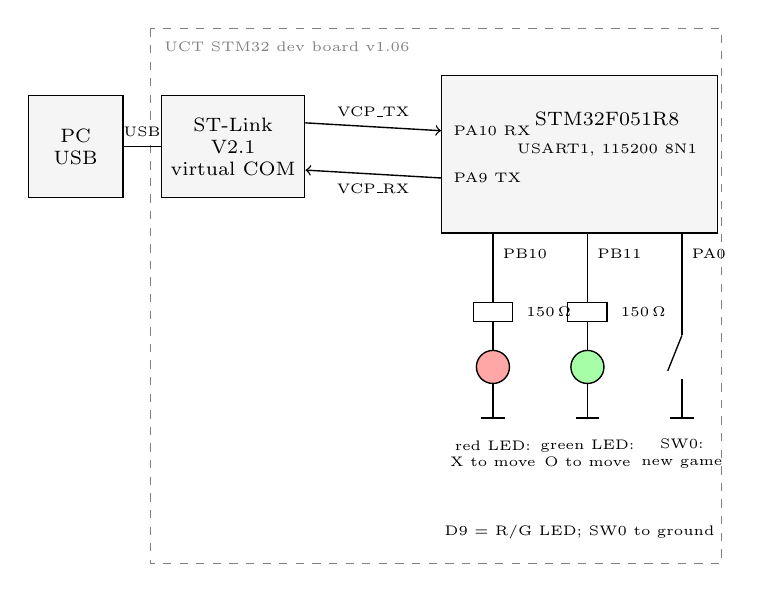
\begin{tikzpicture}[font=\scriptsize,line width=0.5pt,
  box/.style={draw,align=center,fill=gray!8},
  res/.style={draw,minimum width=0.5cm,minimum height=0.24cm,fill=white,inner sep=0pt}]
  \draw[dashed,gray] (1.55,1.5) rectangle (8.8,-5.3);
  \node[anchor=north west,font=\tiny,gray] at (1.6,1.45) {UCT STM32 dev board v1.06};
  \node[box,minimum width=1.2cm,minimum height=1.3cm] (pc) at (0.6,0) {PC\\USB};
  \node[box,minimum width=1.6cm,minimum height=1.3cm] (stl) at (2.6,0) {ST-Link\\V2.1\\virtual COM};
  \node[box,minimum width=3.5cm,minimum height=2.0cm] (mcu) at (7.0,-0.1) {};
  \node at (7.35,0.35) {STM32F051R8};
  \node[font=\tiny] at (7.35,-0.05) {USART1, 115200 8N1};
  \draw (pc.east) -- node[above,font=\tiny]{USB} (stl.west);
  \draw[->] ([yshift=0.3cm]stl.east) -- node[above,font=\tiny]{VCP\_TX} ([yshift=0.3cm]mcu.west);
  \draw[<-] ([yshift=-0.3cm]stl.east) -- node[below,font=\tiny]{VCP\_RX} ([yshift=-0.3cm]mcu.west);
  \node[font=\tiny,anchor=west] at ([xshift=1pt,yshift=0.3cm]mcu.west) {PA10 RX};
  \node[font=\tiny,anchor=west] at ([xshift=1pt,yshift=-0.3cm]mcu.west) {PA9 TX};
  % LED and button
  \foreach \x/\pin in {5.9/PB10,7.1/PB11,8.3/PA0} {
    \draw (\x,-1.1) -- (\x,-1.9);
    \node[font=\tiny,anchor=south west] at (\x,-1.55) {\pin};
  }
  \foreach \x/\col/\cap in {5.9/red/{red LED:\\X to move},7.1/green/{green LED:\\O to move}} {
    \node[res] at (\x,-2.1) {};
    \draw (\x,-1.9) -- (\x,-1.97); \draw (\x,-2.23) -- (\x,-2.6);
    \node[draw,circle,minimum size=0.42cm,inner sep=0pt,fill=\col!35] at (\x,-2.8) {};
    \draw (\x,-3.01) -- (\x,-3.45);
    \draw (\x-0.15,-3.45) -- (\x+0.15,-3.45);
    \node[font=\tiny,align=center] at (\x,-3.9) {\cap};
  }
  \node[font=\tiny,anchor=west] at (6.2,-2.1) {150\,$\Omega$};
  \node[font=\tiny,anchor=west] at (7.4,-2.1) {150\,$\Omega$};
  % button to ground
  \draw (8.3,-1.9) -- (8.3,-2.4); \draw (8.3,-2.4) -- (8.12,-2.85); \draw (8.3,-2.95) -- (8.3,-3.45);
  \draw (8.15,-3.45) -- (8.45,-3.45);
  \node[font=\tiny,align=center] at (8.3,-3.9) {SW0:\\new game};
  \node[font=\tiny] at (7.0,-4.9) {D9 = R/G LED; SW0 to ground};
\end{tikzpicture}

\caption{Circuit: UART link to the PC, the LED and the button.}
\label{fig:circuit}
\end{figure}
